\documentclass[../ClassicThesis.tex]{subfiles}
\begin{document}

%************************************************
\chapter{Joint Computation}\label{ch:joints}
%************************************************

% Use active Voice (we do….)
% Ein Gedanke pro Paragraph
% Terminologie anpassen über alle Arbeiten hinweg (was ist eine Plate für alle…)
% Jeder sollte eine kleine Related Work section haben
% Erklärungen zu warum dieser Algorithmus genutzt wurde und nicht ein anderer + limitations des gewählten Algorithmus
% Hübsche Bildchen zum anschaulichen Erklären!! (ebenfalls konsistent halten: gleich geformte labels etc.)

\section{Joint computation}

\subsection{Volume based clipping}
\paragraph{prerequisite: plategraph intersection lines}

\subsection{Female Joint Computation}
\subsection{Male Joint Computation}

\subsection{Different Fingerjoint types}
TODO: Bilder noch so anpassen, dass nur females/males zu sehen und in echt, wie sie zusammen stecken
\subsubsection{Fingerjoint template}
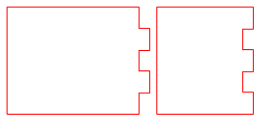
\includegraphics[width=0.5\columnwidth]{Images/fingerjoints.png}
\paragraph{How these joints look like}
\paragraph{How these joints work, and for what material}

\subsubsection{JimJoint template}
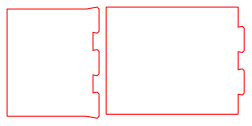
\includegraphics[width=0.5\columnwidth]{Images/jimjoints.png}
\paragraph{How these joints look like}
\paragraph{How these joints work, and for what material}
paper or other easily bendable/eindrueckbar material

\subsubsection{Schwalbe template}
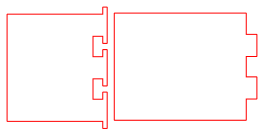
\includegraphics[width=0.5\columnwidth]{Images/schwalbe.png}
\paragraph{How these joints look like}
\paragraph{How these joints work, and for what material}

\subsection{adjusting fingerjoints length when plates are angled}
\paragraph{Deus}

\subsection{Alternative solutions}


\section{Future work}

\end{document}